\section{Experiments and Evaluation}
\label{sec:evaluation}
In Chapter~\ref{sec:implementation}, we detailed our network architecture and its implementation. In this chapter, we study how our network performs given the datasets presented in Chapter~\ref{sec:datasets}. We present and discuss the results of training the outlined neural network architecture for spoken-language identification. We perform an evaluation on our system, while assessing several performance metrics.

Further, we experiment with modified model architectures to maximize the model's accuracy, improve its noise robustness and study the effect of background music on the neural network. To assess the real-world performance of the LID system, we augment our data to simulate various noisy environments. Lastly, we evaluate the classification performance of our approach and discuss the system's interlanguage discrimination capabilities and extensibility to other languages.

\subsection{Hardware Resources}
\label{sec:hardware}
	In order to facilitate Keras's and TensorFlow's hardware-accelerated computation, we executed all training runs on CUDA-compatible\footnote{\url{https://developer.nvidia.com/cuda-zone}, accessed 30 January 2017} \ac{gpu} machines at our disposal at the Internet Technologies and Systems chair of the Hasso Plattner Institute. Details are shown in Table~\ref{tab:hardware}.

	\begin{table}[bp]
	\centering
	\begin{tabu}{lll}
	\toprule
	  		& \textbf{Machine A} 					& \textbf{Machine B} \\ \midrule
	\textbf{OS}  	& Ubuntu Linux 14.04 		& Ubuntu Linux 16.04 \\
	\textbf{CPU}  	& Intel Core i7-4790K at \SI{4.0}{\giga\hertz} & AMD FX-8370 at \SI{4.0}{\giga\hertz} \\
	\textbf{RAM}  	& \SI{16}{\giga\byte} 						& \SI{32}{\giga\byte} \\
	\textbf{GPU}  	& Nvidia GeForce GTX~980 	& Nvidia Titan X \\
	\textbf{VRAM}  	& \SI{4}{\giga\byte} 						& \SI{12}{\giga\byte} \\
	\bottomrule
	\end{tabu}
	\caption{Hardware resources used in training the neural networks. We made heavy use of modern GPUs to benefit from hardware-accelerated numerical computations.}
	\label{tab:hardware}
	\end{table}


\subsection{Data}
\label{sec:data}
	For our performance evaluation, we use the European Speech Repository and YouTube News dataset, as described in Chapter~\ref{sec:datasets}. Both datasets were preprocessed and converted to spectrogram images (see Section~\ref{sec:data_processing}). Each spectrogram image represents a nonoverlapping ten-second snippet of a source audio file. We chose this duration in reference to the NIST LRE2015 challenge~\cite{lre2015}. We split both datasets into a training (\SI{70}{\percent}), a validation \SI{20}{\percent}, and a testing set \SI{10}{\percent}, and all files were distributed equally between all four language classes. The number of samples per class was limited by the language with the least number of files to ensure an equal distribution across the classes. The European Speech repository yields a total of about \num{19000}~training images, which amounts to roughly \num{53}~hours of speech audio. The YouTube News dataset is considerably larger and yields a total of about \num{194000}~training files, or \num{540}~hours. Table~\ref{tab:data_splits} contains the detailed dataset splits.
%
	\begin{table}[bp]
	\centering
	\begin{tabu}{lrr}
	\toprule
	  				& \textbf{European Speech Repository} & \textbf{YouTube News}\\ \midrule
	\textbf{Training Set}    & \num{18788}						 & \num{193432} \\
	\textbf{Validation Set}  & \num{5372}						 & \num{55272} \\
	\textbf{Test Set}        & \num{2684}						 & \num{27632} \\
	\midrule
	\textbf{Total}           & \num{26844}						 & \num{276336} \\
	\bottomrule
	\end{tabu}
	\caption{The number of samples for our training (\SI{70}{\percent}), validation (\SI{20}{\percent}), and testing (\SI{10}{\percent}) sets taken from the two studied datasets.}
	\label{tab:data_splits}
	\end{table}

	Given the European Speech Repository's smaller size, we only used it initially to confirm the validity of our approach. At the point at which we were satisfied with the results, we did not include it in the extensive robustness tests that we used for the evaluation on the YouTube News dataset. Moving on to a bigger challenge, we augmented the original audio of the YouTube News dataset with three different background noises to evaluate how well our model performs in nonideal, real-world situations outside of a news broadcasting studio. For the first experiment, we added generic white noise to the data. For the second experiment, we added noise to simulate an old phone line or bad internet connection during a voice chat. In a last experiment, we added background music to the data. All experiments are described in detail below.


\subsection{Training the Neural Network Model}
\label{sec:training}
	Neural networks have a multitude of hyperparameters that influence the training results drastically. In this section, we briefly explain our choice of hyperparameters alongside other important training settings.

	\begin{description}
	\item[Optimizer] We use \emph{adaptive moment estimation} (Adam)~\cite{kingma2014adam} as our optimization method to quickly and efficiently reach convergence of our model. Adam utilizes momentum during gradient updates to support a quicker convergence. We set the optimizer's parameters $\beta_1$ to \num{0.9}, $\beta_2$ to \num{0.999}, and $\epsilon$ to \num{e-8}. For the majority of trainings, we use Adam and only resort to plain stochastic gradient descent during fine-tuning when we need more control over the learning rate schedule and want smaller weight updates.
	\item[Weights Initializer] All layer weights are initialized within the range $[0, 1]$ using a normalized \emph{Glorot uniform initializer} (also known as \emph{Xavier initializer})~\cite{glorot2010understanding}. This heuristic is designed as a compromise between the two goals of initializing all layers with the same activation or gradient variance, respectively. Thus, the biases are initialized with \num{0} and the weights $\matsym{W}$ of each layer with the following heuristic~\cite[p.~303]{Goodfellow-et-al-2016}:
	$$\matsym{W} \sim U\left(-\frac{6}{\sqrt{n_j + n_{j+1}}}, \frac{6}{\sqrt{n_j + n_{j+1}}}\right)$$
	where $U(-a, a)$ is the uniform distribution in the interval $[-a, a]$ and $n_j$ and $n_{j+1}$ are the sizes of the previous and current layer, respectively.
	\item[Data Normalization] The grayscale images are loaded using SciPy and normalized to values in the range of $[0, 1]$. The shape of all inputs needs to be uniform across all samples and is set to $500 \times 129 \times 1$, unless otherwise noted. Data loading is handled through Python generators to keep the system's memory footprint low.\footnote{\url{https://docs.python.org/3/glossary.html\#term-generator}, accessed 30 January 2017}
	\item[Learning Rate] We set the initial learning rate to~\num{0.001}. Given the Adam optimizer's dynamic adaptation of the learning rate, we expect the learning rate to be automatically increased or decreased after every iteration. Therefore, we do not specify a manual learning rate decay schedule.
	\item[Batch Size] We specify the batch size depending on the available VRAM of the training machine. We use \num{64}~images per batch for Machine~A and \num{128}~images per batch for Machine~B (see Section~\ref{sec:hardware} for the hardware specifications).
	\item[Weight Regularization] comprises any modification we make to a learning algorithm that is intended to reduce its generalization error but not its training error. We employ the L\textsuperscript{2} norm~\cite[p.~231]{Goodfellow-et-al-2016} (sometimes also known as \emph{weight decay}) as a weight regularizer for all convolutional and fully-connected layers to improve the model's generality. This regularization strategy drives the weights closer to the origin by adding a regularization term to our loss function. We penalize the loss value with a weight decay value of \num{0.001}. Additional regularization happens through the use of batch normalization layers.
	\item[Epochs] We limit the model training phase to a maximum of \num{50}~epochs when using the Adam solver. We usually reach convergence well below this threshold. For training sessions with SGD, we increas this parameter considerably, since the weight updates per epoch are smaller, and more training iterations are needed to reach convergence. To speed up our workflow, we employ an early-stopping policy and stop training if the validation accuracy and loss value do not considerably change within a ten-epoch window.
	\item[Metrics] We observe loss, accuracy, recall, precision, and F1 score for both the training and validation set while training the model. All values were are to log files and visualized as graphs in TensorBoard. A complete summary of all assessed metrics can be found in Section~\ref{sec:metrics}.
	\item[Loss] As is common for multivariate classifications, all models are trained with a softmax cross-entropy loss function.
	\end{description}


\subsection{Evaluation}

\subsubsection{Evaluation Metrics}
\label{sec:metrics}
In this section, we discuss the evaluation metrics used throughout our experiments. All metrics are generally defined for binary classification scenarios only. Given our multiclass classification problem, we report the average of the individual class performance measures in the following sections.

\begin{description}
    \item[Accuracy] is a common measure in machine learning and is defined as the ratio of correctly classified samples to all samples in the dataset. In the context of language identification, this translates to:

	$$
	\operatorname{accuracy} = \frac{
	   \vert \{ \text{correctly identified language samples} \} \vert
	  }{
	   \vert \{ \text{all language samples} \} \vert
	  }
	$$

    \item[Precision and Recall] \emph{Precision} defines the proportion of retrieved language samples that are correctly identified as belonging to said language. \emph{Recall} is the fraction of correctly identified language samples to all samples belonging to this language. Both measures are calculated using true and false positives as well as false negatives. These are defined as follows. \emph{True positives} are the samples that are correctly attributed to a given language. In contrast, \emph{false positives} are attributed to a given language, but they actually do not belong to it. Lastly, \textit{false negatives} are, by mistake, not recognized as part of a given language.

	    $$
	    \operatorname{precision} = \frac
	      {\operatorname{true} \operatorname{positives}}
	      {\operatorname{true} \operatorname{positives} + \operatorname{false} \operatorname{positives}}
	    $$

		$$
		\operatorname{recall} = \frac
			{\operatorname{true} \operatorname{positives}}
			{\operatorname{true} \operatorname{positives} + \operatorname{false} \operatorname{negatives}}
		$$


    \item[The F1 Score] is the scaled harmonic mean of precision and recall. It is a combined judgement of both values, since it is generally not interesting to assess one without the other.

    	$$
    	\operatorname{F1} = 2 * \frac{\operatorname{precision} * \operatorname{recall}}{\operatorname{precision} + \operatorname{recall}}
    	$$

\end{description}

\subsubsection{Results for the EU Speech Repository Dataset}
\label{sec:results_eu}
In order to verify our theoretic model of using convolutional neural networks for classifying audio data in the image domain, we established a baseline with the smaller EU Speech Repository dataset. Previous work with CNNs showed that a careful arrangement of the neural network layers has great effect on the final classification performance. If one does not use enough or sufficiently large layers, the model is not able to properly distinguish between classes. Going too deep or using too large layer outputs increases the overall number of model parameters to a degree where both training time and classification performance suffer again. The goal of this experiment is to find favorable settings for the number of necessary convolutional layers, the kernel sizes of the convolutions, the numbers of output maps of the convolutional layers, and finally, the number of hidden units of the fully-connected layer.

	In Section~\ref{sec:cnn_architecture}, we introduced three proposals for different CNN architectures. CNN\_A features large kernel sizes in the first two layers, and we expect this architecture to capture more information up-front. A slightly smaller version of this design with less parameters is CNN\_B. It serves as an assertion to verify that the number of output feature maps of CNN\_A is properly sized and not too large. Lastly, CNN\_C features equally-sized kernels and boasts both more convolutional layers as well as an increased number of feature map outputs.

CNN\_A outperforms both of the other network architectures with respect to all the evaluated performance measures, as shown in Figure~\ref{fig:eu_results}.
%
	\begin{figure}[tp]
  		\centering
    	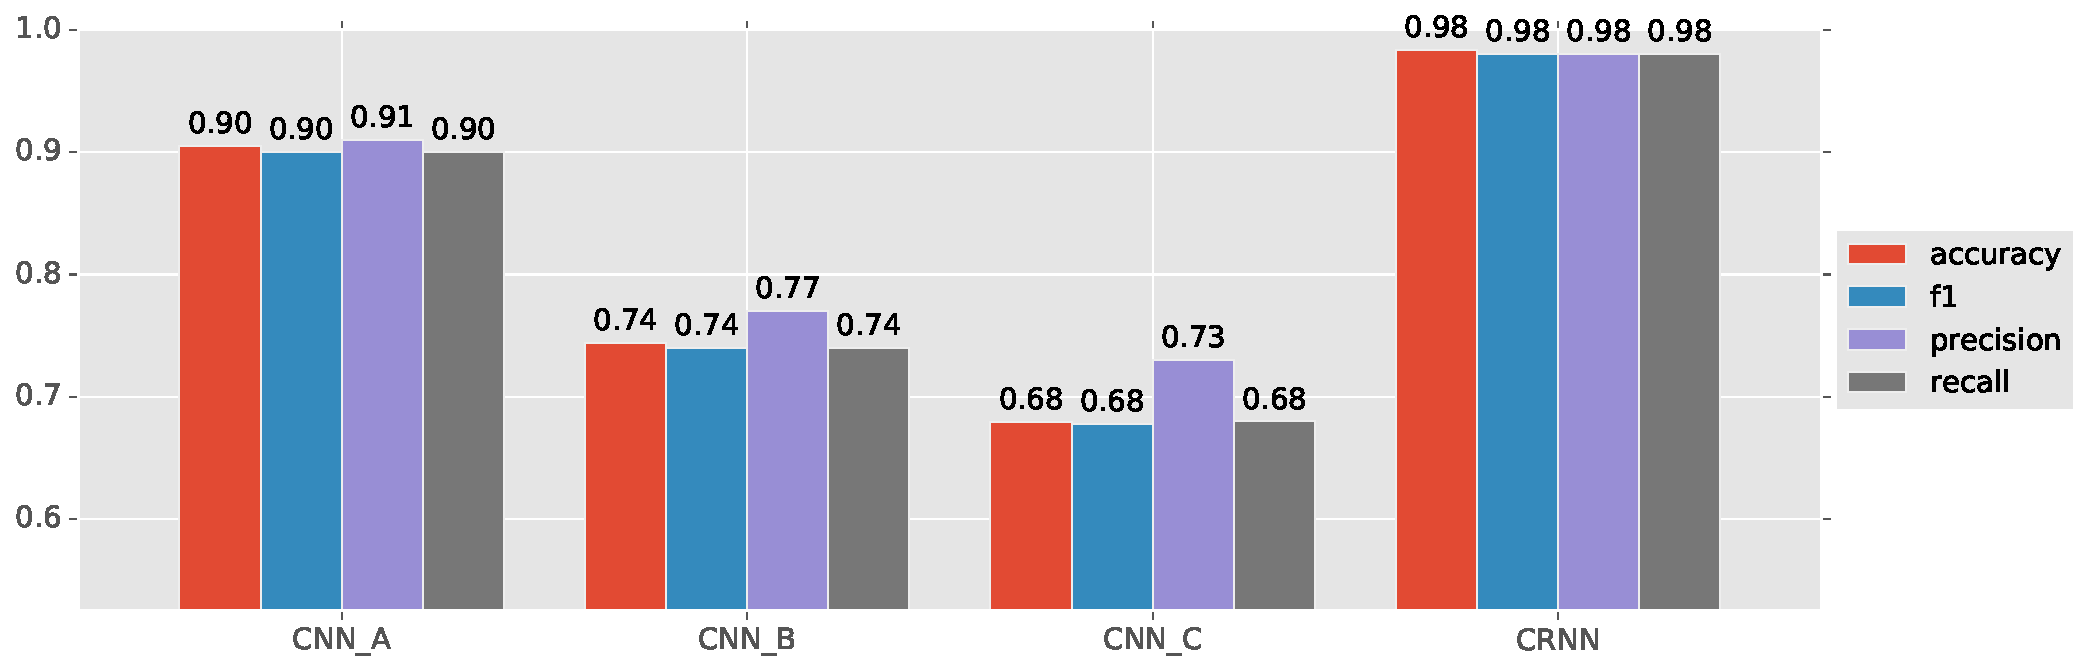
\includegraphics[width=\textwidth, keepaspectratio]{plots/results_eu_plot.pdf}
    	\caption{Performance measure comparison of three different CNN architectures and our proposal of a \ac{crnn} model evaluated on the EU Speech Repository dataset. CNN\_A outperforms all other CNN approaches with a top accuracy of \num{0.90}, but is bested by \num{0.98} accuracy with CRNN, showing the potential of the approach developed in this thesis.}
    	\label{fig:eu_results}
	\end{figure}
%
With a top-1 accuracy of \num{0.90}, CNN\_A trumps CNN\_B and CNN\_C with \num{0.74} and \num{0.68}, respectively. Comparing the F1 score, we get a very similar result: \num{0.90} versus \num{0.74} and \num{0.68}. This experiment confirms a few of our initial hypotheses (as outlined in Section~\ref{sec:task-specification}). First, convolutional neural networks are a successful technique for classifying speech audio data. Second, spectrogram images are meaningful representations for audio and retain enough information for language identification. Third, larger kernels for the initial convolutional layers are, indeed, favorable, since the increased receptive field captures both the time and the frequency domain better.

Based on these findings, we did further experimented with CNN\_A. Mishkin et al. were able to gain a small improvement in accuracy by exchanging the convolutional layers' activation functions~\cite{mishkin2016systematic}. For this purpose, we replaced our ReLU activations with \emph{exponential linear units} (ELU)~\cite{clevert2015fast} but were unable to measure any improvement (with only \num{0.85} accuracy).
Shi et al. proposed to use $1 \times 2$ rectangular pooling windows instead of the conventional square ones~\cite{shi2016end}. This tweak yields feature maps with larger width and, hence, more features along the time domain. In theory, this should increase the CNN's sensitivity to occurrences of frequencies at certain time intervals. For this experiment, we were unable to improve (\num{0.81} accuracy), but we come back to this technique for our CRNN approach in Section~\ref{sec:duration}.

The task of this thesis is to evaluate the use of deep convolutional recurrent networks for language identification. Therefore, we extend our previously best-performing CNN\_A with a bidirectional \ac{lstm} layer to capture time steps both forward from the start and backward from then end of an audio segment. Our model interprets the \ac{cnn} output as an intermediate high-dimensional representation of the audio frequencies. Every vector entry along the $x$~axis is used as a single time step and input to the LSTMs, as explained in Section~\ref{sec:hybrid_networks}. Confident in the features captured by our convolutional layers, we freeze them during the CRNN training phase to disable any further weight updates for these layers. Instead, we focus on training only the LSTMs weights and learning the frequency sequences of the audio samples. Our bidirectional LSTM layer trains two individual LSTMs with \num{512}~outputs each, one moving forward along the input sequence and one backward. Both outputs are concatenated to form a single output vector with a dimension of \num{1024}, which is followed by a single, fully-connected layer for classification.

Our CRNN architecture outperformed all CNN approaches significantly. A top-1 accuracy of~\num{0.98} and an F1 score of~\num{0.98} prove the viability of the CRNN approach and reaffirm the central hypothesis of this thesis.


\subsubsection{Effect of Audio Duration}
\label{sec:duration}
In all previous experiments, we split the audio recordings into ten-second segments, which translates to an image dimension of $500 \times 129$ pixels in the spectrogram. We decided on ten-second audio snippets to replicate the setup of the \ac{nist} LRE~2015 challenge~\cite{lre2015}. To study the effect of audio duration on classification performance, we set up two versions of the EU Speech Repository dataset with nonoverlapping five- and \num{20}-second snippets but left the number of frequency bins unchanged. Hence, we change the input dimensions to $250 \times 129$ pixels and $1000 \times 129$ pixels, respectively, and cannot just reuse our previously trained models but have to train new models.

As a baseline, we use the same CNN\_A architecture as explained in Section~\ref{sec:cnn_architecture}. When completely training the five-second version from scratch, we achieve an accuracy of~\num{0.81}, falling short of the results achieved with the ten-second snippets. Next, we apply some transfer learning and fine-tune CNN\_A on the five-second dataset. Since the convolutional layers are not bound to a specific input size and given that the frequency features do not change in dimension, we are able to reuse all the convolutional weights. For fine-tuning, we freeze the convolutional layers, confident in their ability to detect frequency features, and only retrain the final two fully-connected layers. After bisecting the input data, the amount of model parameters is greatly reduced, especially the fully-connected layer weights. To account for this, we fine-tune one model with a fully-connected layer of \num{512}~outputs and a second one with the default \num{1024}~outputs. Overall, this yields an accuracy of~\num{0.88} and~\num{0.89}, respectively. We conclude that the effect of the smaller fully-connected layer is only marginally better.

After establishing a solid CNN foundation, we apply the same CRNN approach as previously highlighted. Due to the shorter audio duration, the final pooling layer only features five output units along the $x$ axis, compared to the \num{13}~output units of the ten-second CRNN. When interpreted as a sequence of time steps and fed into the bidirectional LSTM, the accuracy improves only marginally to \num{0.90}. We suspect that the number of time steps is too little to take full advantage of the recurrent network layer.

In an effort to increase the number of output units of the final pooling layer and, hence, increase the sequence length, we apply the $1 \times 2$ rectangular pooling tweak again. We change the final two pooling layers and increase the number of output units along the $x$ axis to \num{22}. The $y$ axis remains unaffected. The resulting accuracy of~\num{0.90} and the F1~score of~\num{0.91} remain comparable to the previous model and do not achieve improvements.

For the twenty-second version, we train the network from scratch using the CNN\_A architecture. This yields an accuracy of \num{0.90}, which is comparable to the ten-second counterpart. This experiment uses double the amount of pixels along the $x$ axis as the ten-second baseline. This expansion of data leads to an increased computation time. Additionally, we feel that our LID system is less flexible when using longer input audio snippets. We conclude that these longer snippets do neither improve the accuracy nor make the LID system more attractive overall.

In summary, we believe that both decreasing and increasing the duration of the audio snippets used for training has a negative effect on the classification performance. While it is possible to train and fine-tune CNNs matching their ten-second counterparts accuracy-wise, we find that the CRNN approach does not boost the model effectiveness in a similar manner.
Table~\ref{tab:audio_duration} shows the results of our experiments with varying sample durations, confirming that the 10-second CRNN performed best in our evaluation.
%
	\begin{table}[tp]
	\centering
	\begin{tabu}{lcc}
	\toprule
  \textbf{Model Architecture}                            & \textbf{Accuracy}  & \textbf{F1 Score}   \\ \midrule
  CNN (\SI{5}{\second}), from scratch                              & 0.81      & 0.81 \\
  CNN (\SI{5}{\second}), fine-tuned with \num{1024}~fully-connected units & 0.88      & 0.89 \\
  CNN (\SI{5}{\second}), fine-tuned with \num{512}~fully-connected units  & 0.89      & 0.89 \\
  CNN (\SI{20}{\second}), from scratch                             & 0.90      & 0.90 \\
  CRNN (\SI{5}{\second}), with \num{5}~time steps                        & 0.90      & 0.91 \\
  CRNN (\SI{5}{\second}), with \num{22}~time steps                       & 0.90      & 0.91 \\ \midrule
  CRNN (\SI{10}{\second}), for reference                           & 0.98      & 0.98 \\
 	\bottomrule
	\end{tabu}
	\caption{Various CNN and CRNN model configurations trained on audio samples with durations of \num{5}, \num{10}, and \num{20}~seconds. The ten-second CRNN outperforms the other configurations with an accuracy and F1 score of \num{0.98} and \num{0.98}, respectively.}
	\label{tab:audio_duration}
	\end{table}


\subsubsection{Results for the YouTube News Dataset}
\label{sec:results_news}
Following the promising results from the experiments with the EU Speech Repository, we switch to the ten-times larger YouTube News dataset for further training and evaluation.

For our first experiment, we use the same CNN\_A architecture as before but initialize the model weights with the weights of the best-performing model of the EU Speech Repository evaluation. Our reasoning here is to reuse the convolutional layers that are already trained to identify frequency features. However, with an accuracy of only~\num{0.79}, CNN\_A does not perform as well as anticipated. One reason for this could be that the EU dataset is a lot smaller and does not feature as many diverse situations as present in news broadcasts. In the case of broadcasts, all audio is recorded in a similar environment without much background noise and exhibits high signal quality.

Next, we train the same CNN completely from scratch with randomly initialized weights. We had several setbacks when using an Adam optimizer and reverted to using standard SGD to keep the loss value in check. Specifically, we encountered the \emph{exploding gradient problem}~\cite[p.~288]{Goodfellow-et-al-2016} and had to use \emph{gradient clipping} to solve the issue. With this tweak, we are able to get the model to converge and achieve an accuracy of~\num{0.9090}, besting our previous attempts.

Given the larger size of the new dataset, we also tried to increase the number of parameters by doubling the feature maps of the convolutional layers. This, however, did not help. As a next step, we applied the CRNN approach again. Based on this CNN, we added our bidirectional LSTM layers in the same manner as for the previous CRNNs and were able to slightly improve both our accuracy and F1~score to~\num{0.91}.

To evaluate how our model architecture fares against established deep learning models, we train a model using Google's Inception-v3 layout~\cite{szegedy2016rethinking}. This network design features more layers and is considerable deeper than our proposed CRNN architecture and is the result of Google's latest research into neural networks for image recognition tasks. Instead of a monolithic network design of sequential layers, Inception-v3 uses a combination of parallel inception units, a sequence of convolution layers, as one building block. Evaluating the Inception-v3 model results in a top accuracy of~\num{0.9488}, improving our results significantly. Applying the established CRNN treatment to this model increased the performance to an accuracy of~\num{0.9579}. In order to boost the performance even further, we also try a CRNN variation, where both the convolutional layer weights and the LSTM weights are trained jointly. In contrast to our initial CRNN approach, this method also updates the existing convolutional filters. We find, however, that this variation does not improve performance. Figure~\ref{fig:news_results} shows an overview of the performance metrics of the mentioned experiments.
%
	\begin{figure}[tp]
  		\centering
    	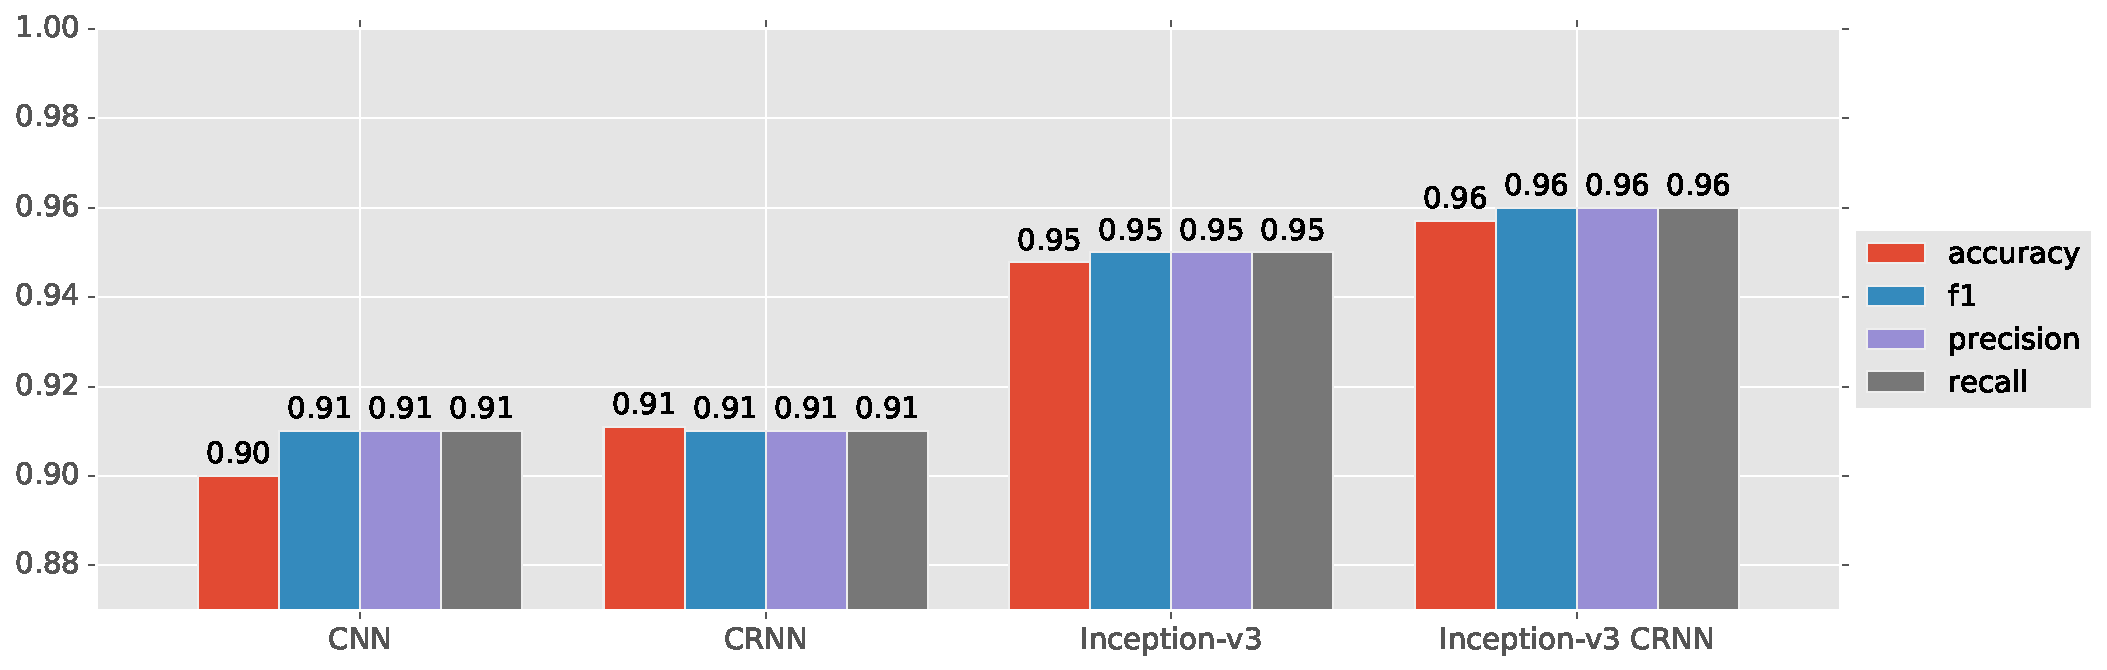
\includegraphics[width=\textwidth, keepaspectratio]{plots/results_news_plot.pdf}
    	\caption{Performance measurement comparison between our CNN and CRNN models and Inception-v3-based models. With a top accuracy of~\num{0.96}, the Inception-like CRNN performs best but needs more than five times the number of parameters compared to our proposed model architecture.}
    	\label{fig:news_results}
	\end{figure}
%
The increased performance, however, does not come without a cost. With a total of \num{3153924} parameters, our CRNN uses roughly six times less parameters than the Inception-v3 CRNN with its \num{19}~million parameters. This increases training time, requires more training data, and consumes more GPU memory. On disk, the serialized model weights come in at \SI{30}{\mega\byte} versus \SI{260}{\mega\byte}, which could be a potential disadvantage for deployment on mobile phones.



\subsubsection{Interlanguage Discrimination}
\label{sec:lang_discrimination}

Previous work raised concerns about the similarity of our four feature languages---English, German, French, and Spanish---and the model's inability to discriminate between them properly~\cite{montavon2009deep}. Both English and German belong to the West Germanic language family, while French and Spanish are part of the Romance languages. We hypothesized that our deep learning approach to language identification is able to differentiate between them reliably.

The results support our hypothesis. Table~\ref{tab:language_family_crnn} shows the confusion matrix when evaluating language family pairs on the best-performing CRNN.
%
	\begin{table}[tp]
	\centering
	\begin{tabu}{l|cccc}
	      & \textbf{EN}     & \textbf{DE}     & \textbf{FR}     & \textbf{ES} \\ \midrule
    \textbf{EN}  & \cellcolor{lightgray} 6153   & 339    & 181    & 225 \\
    \textbf{DE}  & 426    & \cellcolor{lightgray} 6128   & 173    & 162 \\
    \textbf{FR}  & 200    & 145    &  \cellcolor{lightgray} 6447   & 107 \\
    \textbf{ES}  & 214    & 170    & 115    & \cellcolor{lightgray} 6399 \\
	\end{tabu}
	\caption{Confusion matrix of our best-performing CRNN. Ground truth values are along the rows, predicted values along the columns. English audio files are likely to be misclassified as German and vice versa. Both languages belong the family of Germanic languages.}
	\label{tab:language_family_crnn}
	\end{table}
%
Spanish and French audio files separate very well with hardly any wrong classifications. Both languages are more likely to be classified as German and English rather than as the respectively other one, demonstrating that their learned representations are quite distinctive within their language family.

German and English language samples have a tendency to be confused. Furthermore, English also has a slight bias towards French, an observation in line with related work~\cite{werkmeister2016practical}. With German, however, the classification error is distributed evenly between French and Spanish. Overall, German samples are misclassified most often across all languages.

	The confusion matrix for the Inception-v3 CRNN in Table~\ref{tab:language_family_inception} leads to similar observations as with our CRNN model. Again, German exhibits the most classification errors.
%
	\begin{table}[tp]
	\centering
	\begin{tabu}{l|cccc}
	      & \textbf{EN}     & \textbf{DE}     & \textbf{FR}     & \textbf{ES} \\ \midrule
	  \textbf{EN}  & \cellcolor{lightgray} 6648   & 140    & 45     & 61 \\
	  \textbf{DE}  & 152    & \cellcolor{lightgray} 6639   & 62     & 44 \\
	  \textbf{FR}  & 68     & 59     & \cellcolor{lightgray} 6742   & 27 \\
	  \textbf{ES}  & 75     & 83     & 42     & \cellcolor{lightgray} 6697 \\
	\end{tabu}
	\caption{Confusion matrix of the Inception-v3 CRNN. Ground truth values are along the rows, predicted values along the columns. Despite its deeper architecture, Inception-v3 makes similar types of mistakes as our proposed CRNN.}
	\label{tab:language_family_inception}
	\end{table}


\subsubsection{Noise Robustness}
\label{sec:noise_robustness}
Given that we left the raw audio data unchanged, we expected a certain degree of noise within the dataset. Therefore, we hypothesized that the neural network developed some noise robustness by itself. For instance, the convolution operations of the earlier layers summarize pixel values over an image patch and help with masking noise. To prove our theory, we generate two augmented datasets based on the YouTube News dataset.

For the first augmented dataset, we mix the audio signal with randomly generated white noise sounds. The resulting audio samples are still easily identifiable by human listeners. The noise has a very strong audible presence, so much that human testers are easily annoyed after a few seconds of listening to it.

For the second augmentation, we add a more periodic crackling noise, emulating analog telephony or a bad voice chat connection. We sample a selection of fitting sound effects and randomly apply these to the source signal using the PyDub library.\footnote{\url{https://github.com/jiaaro/pydub}, accessed 01 March 2017} The resulting noise is not as noticeable and less intrusive as the white noise but gives the augmented audio file a subdued vintage quality.

The white noise significantly deteriorates the language identification performance, both for our CRNN proposal and the Inception-v3 CRNN, as can be seen in Table~\ref{tab:noise}.
%
	\begin{table}[tp]
	\centering
	\begin{tabu}{lccccc}
	\toprule
	\textbf{Dataset} & \multicolumn{2}{c}{\textbf{CRNN}} & \multicolumn{2}{c}{\textbf{Inception-v3 CRNN}} \\
                & \textbf{Accuracy}  & \textbf{F1 Score}    & \textbf{Accuracy}  & \textbf{F1 Score}   \\ \midrule
No Noise		& 0.91		& 0.91	& 0.96		& 0.96 \\
White Noise     & 0.63      & 0.63  & 0.91      & 0.91 \\
Crackling Noise  & 0.82      & 0.83  & 0.93      & 0.93 \\
 	\bottomrule
	\end{tabu}
	\caption{Accuracy and F1 score for our models evaluated on the speech data augmented with two different types of noise. Our proposed model architecture is susceptible to noise, and its performance deteriorates. The much deeper architecture of Inception-v3 CRNN is more robust against noise and retains a high performance.}
	\label{tab:noise}
	\end{table}
%
The noise spectrogram in Figure~\ref{fig:noise} show that the white noise effect has a very strong influence on the resulting image.
%
	\begin{figure}[tp]
  		\centering
    	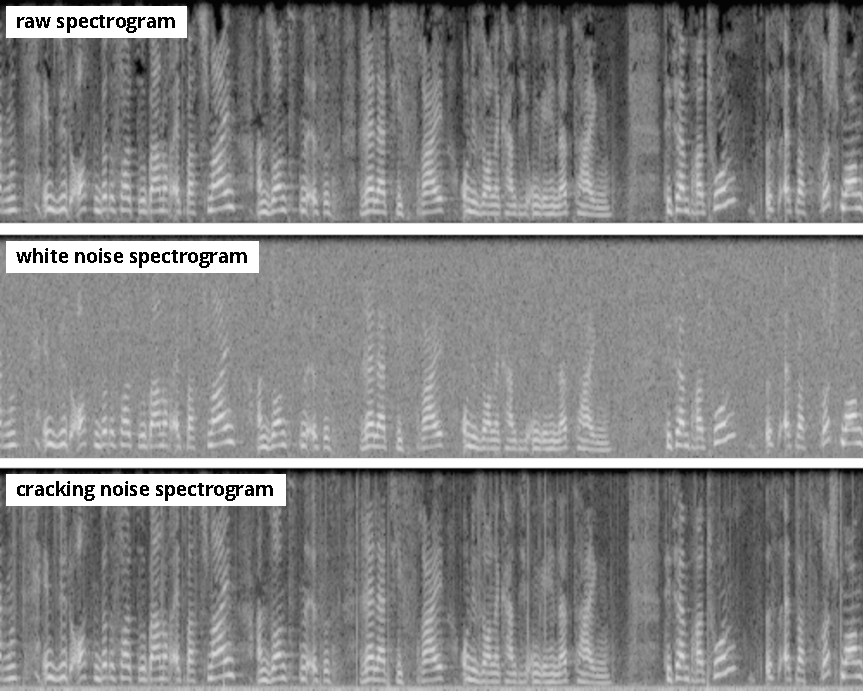
\includegraphics{img/noise_spectrograms.pdf}
    	\caption{Spectrograms generated from the raw data, augmented with white noise and mixed with a crackling noise emulating analog telephony or a bad voice chat connection. The white noise aggressively subdues most higher frequencies and pauses that decrease the classification performance. The crackling noise is less intrusive and, therefore, does not affect accuracy as much.}
    	\label{fig:noise}
	\end{figure}
%
Most parts of the image end up covered by the distinct noise texture and only the lower frequency features remain intact. Yet, most speech frequencies are still contained in this range. All pauses and fine-grained details are also lost to the noise sound. The crackling experiment does not incur such a dramatic drop in performance. That might be in part due to the consistent recurring sound of the noise, in contrast to the randomly generated white noise sound. Perhaps, a second factor is the lower, less intrusive volume used for augmenting this dataset.

The deeper, more complex structure of the Inception-v3 CRNN suffers from a significantly smaller performance deterioration than our proposed CRNN model architecture. The more than five-times higher number of parameters seems to capture the frequency features in a more robust manner. In an attempt to remedy the performance loss of our model, we trained and fine-tuned models containing white noise data. We experimented with a \SI{100}{\percent}~noise dataset and the original YouTube News dataset augmented with \SI{10}{\percent}~white noise. 

While both approaches recover some performance in the white noise setting, they impair language identification in the general test set and the crackling noise environment as a trade-off.

Let it be noted that our audio mixing was fully automated and that the resulting samples varied in speech and noise volume. We tried to match volume levels of speech and noise to maintain as much clarity of speech as possible, yet some samples have an artificial quality to them.



Overall, we note that even deep convolutional recurrent networks are still subject to the influence of noise on audio. We learned that our spectrogram preprocessing method does not help in these situations, and that different network architectures play an important role in dealing with these situations.



\subsubsection{Background Music Robustness}
\label{sec:music_robustness}
	\begin{table}[tp]
	\centering
	\begin{tabu}{lcccc}
	\toprule
\textbf{Dataset} & \multicolumn{2}{c}{\textbf{CRNN}} & \multicolumn{2}{c}{\textbf{Inception-v3 CRNN}} \\
                  & \textbf{Accuracy}  & \textbf{F1 Score}    & \textbf{Accuracy}   & \textbf{F1 Score}   \\ \midrule
\textbf{No Music}		  & 0.91		  & 0.91	  & 0.96	  & 0.96 \\
\textbf{Background Music}  & 0.70      & 0.70  & 0.89  & 0.89 \\
 	\bottomrule
	\end{tabu}
	\caption{Accuracy and F1 score for our models evaluated on the speech data augmented with background music from different genres.}
	\label{tab:background-music}
	\end{table}
Many real-world audio applications involve some form of music. For example, imagine speaking into your mobile phone from a busy caf\'{e} with background music or having a voice chat session at home while the TV is running. Therefore, we evaluate our model to see if language identification is still possible when mixing speech with music. For this experiment, we use two different test sets. For the first series, we augment our existing YouTube News dataset with randomly sampled background music, similar to the background noise augmentation.

The background audio was obtained from Soundcloud, and features royalty-free, instrument-only music from various genres, including Pop, Dubstep, Rock, and Electro.\footnote{\url{https://soundcloud.com/royalty-free-audio-loops}, accessed 01 March 2017} We normalized the volume of these tracks and overlaid them onto our speech data while trying to stay below the speech audio volume. In the best cases, the two audio streams blend nicely with the background music, producing a soft but noticeable ambient effect while retaining the clarity of the speech. In some other cases, audio level and volume of speech or music are over-accentuated. The final result, however, does neither resemble a song nor a piece of music. We changed neither the tempo nor the pitch of our speakers, and the rhythm of the vocals does not match the rhythm of the background audio.


	
Given that our training set does not intentionally include samples with music or songs, we expected the performance to be lower than for pure speech samples. Table~\ref{tab:background-music}, which shows accuracy and F1 score for the two test sets augmented with background music, confirms this hypothesis.

Additionally, it should be noted that the frequency activations of the instruments overlap with the speech frequencies. There is no easy way to separate the instruments from the singer or speaker in a music recording. The approach described here is not intended to work for language identification in songs, and we leave this task open for future work. 
%
	\begin{figure}[tp]
  		\centering
    	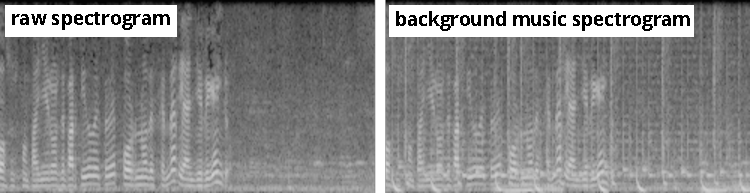
\includegraphics{img/background_music.pdf}
    	\caption{Spectrograms generated from the raw data and augmented with background music noise. The added background music is clearly visible in the resulting spectrogram and changes the classification performance. Note that the previously silent part on the right-hand side now shows frequency activations as well. Additionally, the original ripple-like patterns become a lot more subdued and unclear. Further, new frequency activation patterns along the bottom of the image become visible.}
    	\label{fig:background_music}
	\end{figure}
%

Figure~\ref{fig:background_music} shows the raw and augmented spectrograms of a Spanish speech snippet.
There are several changes of note. First, the large area on the right-hand side, which was formerly silent, starts to show repeated patterns. Second, along the lower image boundary, we see new, regular frequency activation spikes. Third, the clear ripple-like patterns in the raw spectrogram turn into muddy, unclear patterns.

\subsubsection{Model Extensibility}
\label{sec:extensibility}
So far, all our experiments were conducted on datasets consisting of only four languages: English, German, French, and Spanish. We now extend the existing set with two new languages spoken by millions around the globe: Mandarin Chinese and Russian. The goal of this experiment is to learn whether we can expand our model to other languages.

We increase our existing YouTube News dataset with samples taken from Chinese and Russian news channels. Altogether, these now form the Extended YouTube News dataset described earlier in Section~\ref{sec:youtube_news}. In order to maintain the class distribution for six languages, we have to decrease the number of training samples of the existing samples slightly. Table~\ref{tab:dataset_comparison} contains the details for the Extended YouTube News dataset.

For this experiment, we first fine-tune our previously best CNN by replacing the final fully-connected layers and adjust the number of output nodes to accommodate for six classes. The resulting model serves as the basis for training the CRNN in a similar manner as in earlier experiments. Applied on the test set, we measure an accuracy of~\num{0.92} and an F1 score of~\num{0.92}. Both measurements match our previous evaluation with four languages on the YouTube News dataset, proving that the proposed CRNN architecture can be extended to cover more languages. Figure~\ref{fig:6lang} shows individual performance measures for each language.

Mandarin Chinese outperforms all other languages with a top accuracy of~\num{0.96}, which could be explained by its sound contrast to western languages and its unique intonation. We also note that Russian is most frequently misclassified as Spanish and vice versa. In contrast to our previous observation in Section~\ref{sec:lang_discrimination}, German is no longer the worst-performing class but English instead. This is, in part, due to a significant number of misclassifications as Russian samples.
%
	\begin{figure}[tp]
  		\centering
    	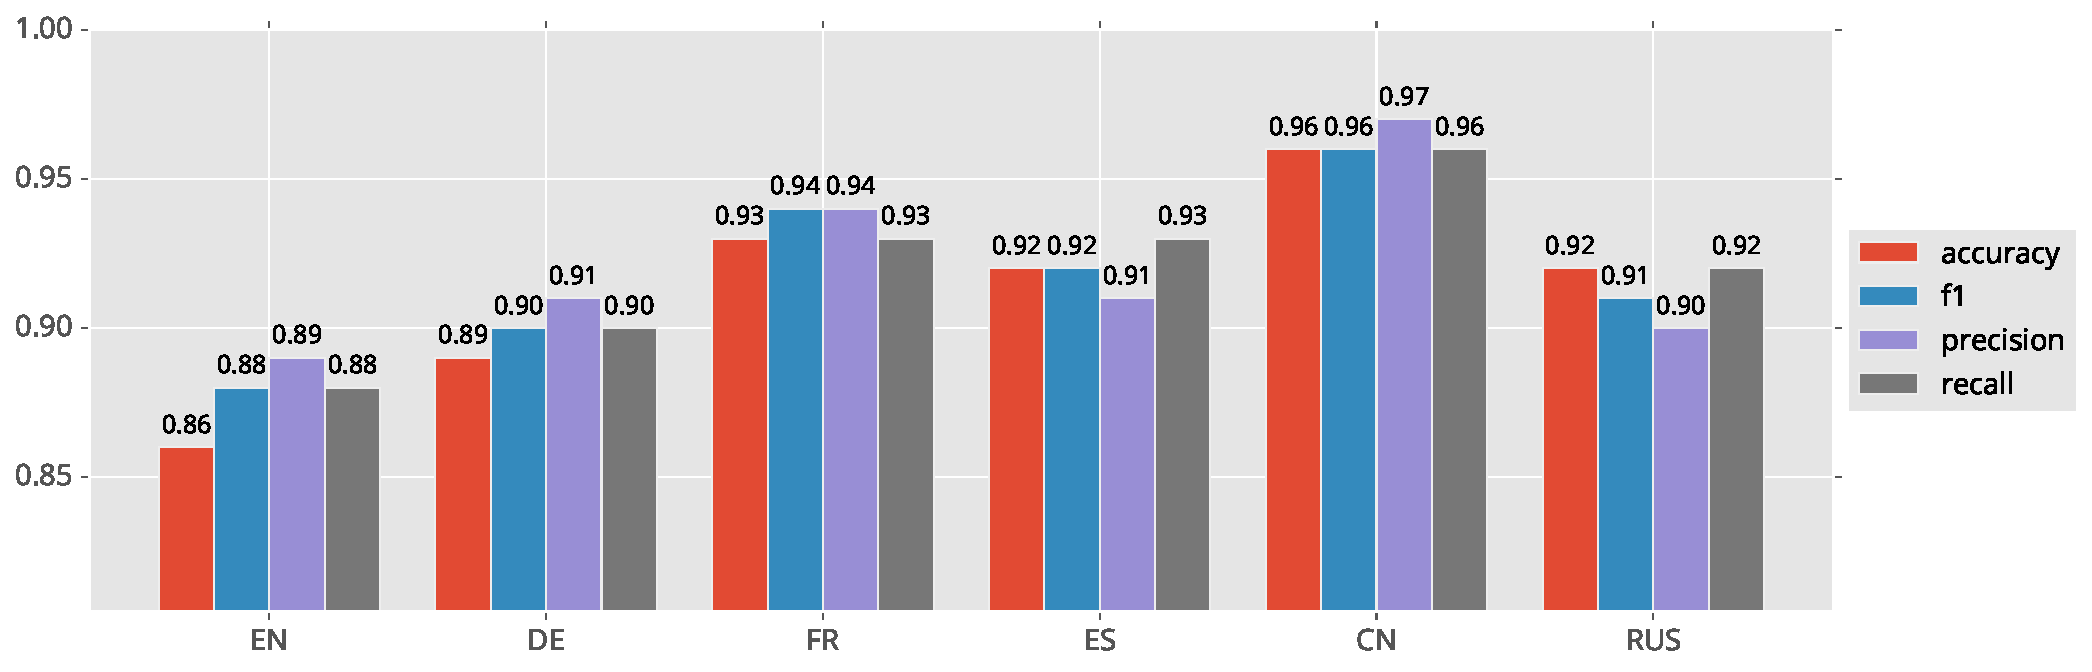
\includegraphics[width=\textwidth, keepaspectratio]{plots/results_6lang_plot.pdf}
    	\caption{Individual performance measurements for each of our six target languages: English, German, French, Spanish, Mandarin Chinese, and Russian. Chinese exhibits the best misclassification rate, while English performs the worst. Overall, the model performance is consistent with the previous evaluations on only four languages, as highlighted in Section~\ref{sec:results_news}.}
    	\label{fig:6lang}
	\end{figure}
%

Given that both new languages are rooted within their own respective language families and feature considerably different intonations, we are content to find that the features learned by our model are, indeed, universal in nature. We believe that the approach to language identification proposed in this thesis can be successfully applied to a wide variety of languages.

\subsubsection{Visualizations}
\label{sec:visualization}
In all previous sections, our model was described and evaluated by measuring various performance indicators and by applying them to different datasets. In this section, we illustrate earlier observations with plots.

First, we visualize the high-dimensional language vector embedding space using the \emph{t-distributed stochastic neighbor embedding} algorithm (\ac{tsne})~\cite{maaten2008visualizing}. t-SNE is a nonlinear dimensionality reduction technique employed to map high-dimensional data onto 2D~or 3D~space for plotting purposes. We apply this machine learning algorithm to the first \num{2000}~predictions of our second-to-last fully-connected layer (right before the classifier) and project our \num{1024}-dimensional YouTube News embeddings into a 2D~space. Figure \ref{fig:tsne} shows the resulting plot, which displays a good separation of our four language classes into independent clusters, confirming that our network learned effective representations of the audio features.
%
	\begin{figure}[tp]
	\centering
	\begin{minipage}{.5\textwidth}
	  \centering
	  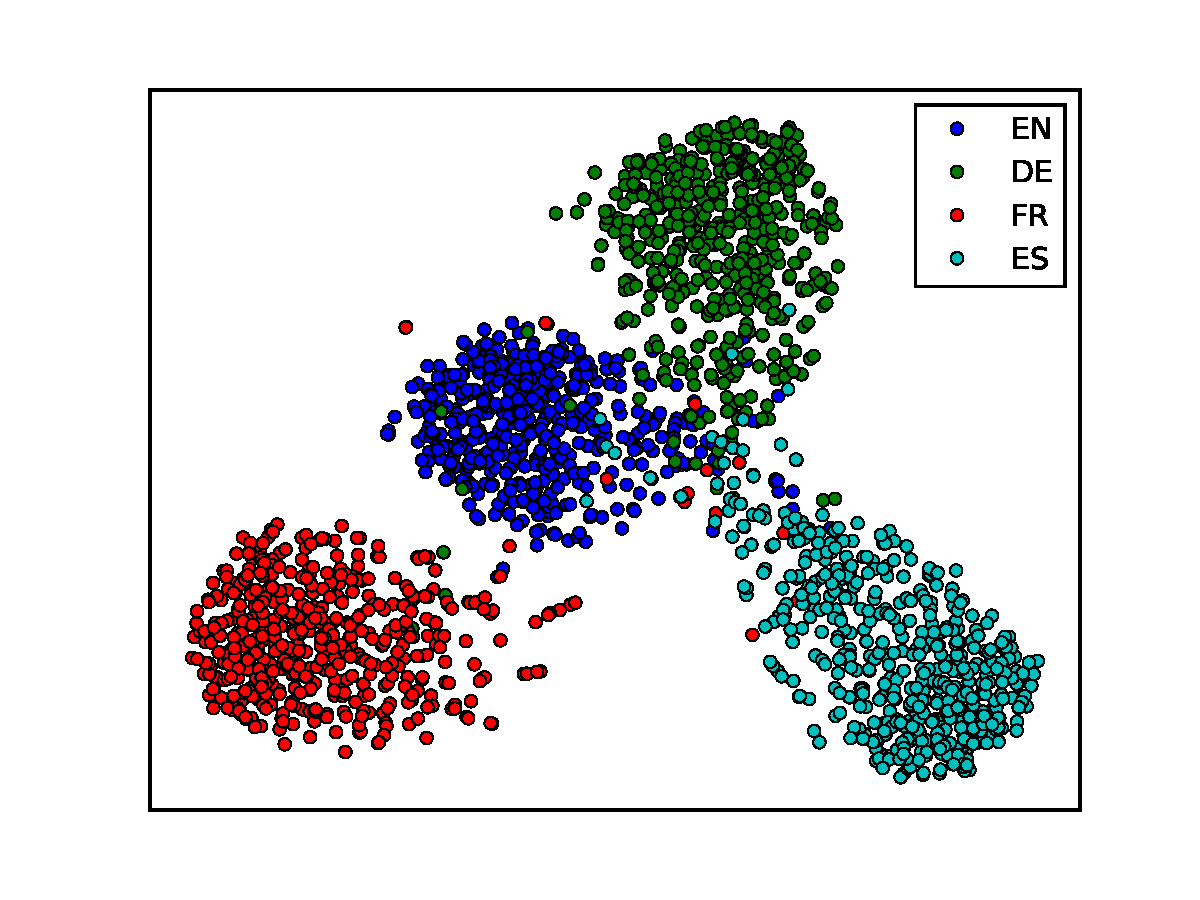
\includegraphics[width=\linewidth]{plots/tsne.pdf}
	\end{minipage}%
	\begin{minipage}{.5\textwidth}
	  \centering
	  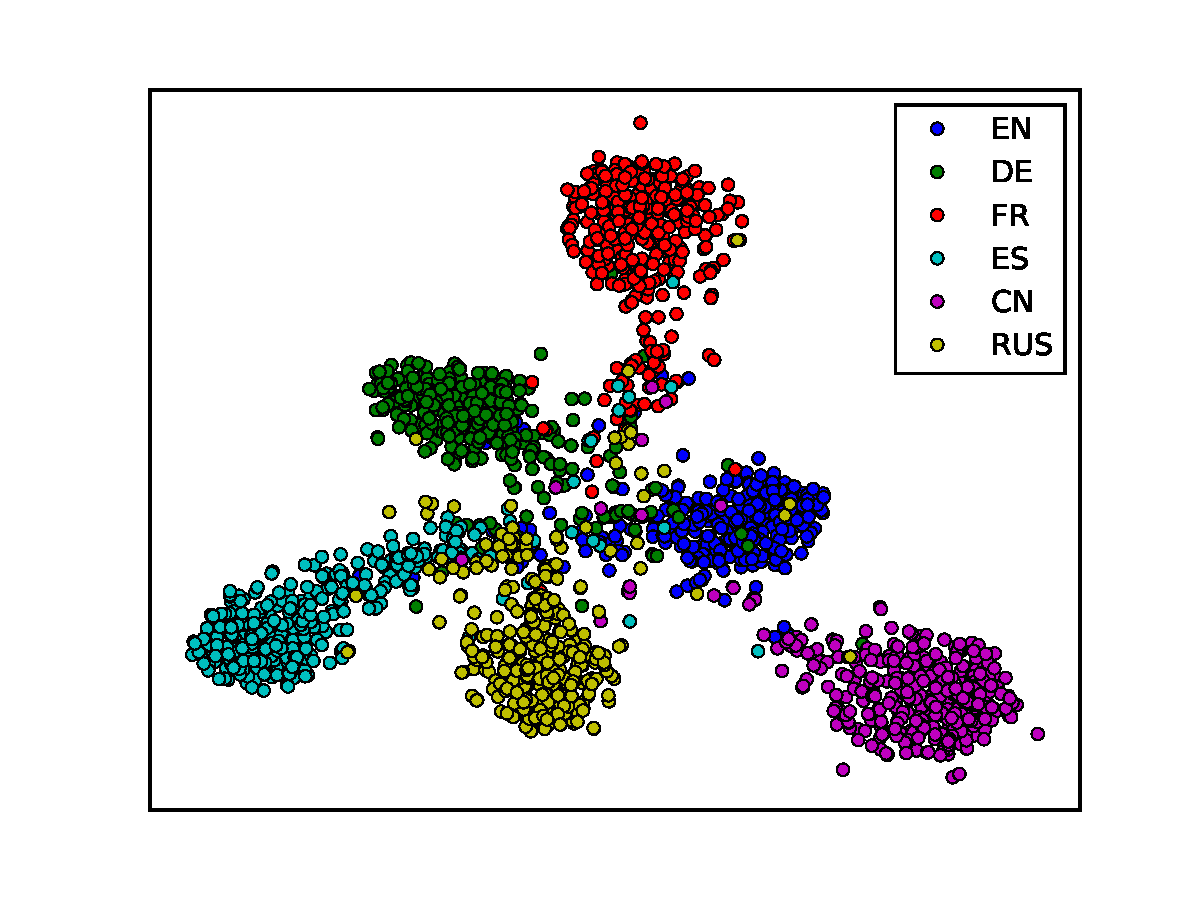
\includegraphics[width=\linewidth]{plots/tsne_6lang.pdf}
	\end{minipage}
	\caption{Two-dimensional t-SNE plots of the high-dimensional vector representation of our YouTube News samples for models trained with four and six languages,  respectively. All language classes form distinct clusters, confirming that our networks learned effective representations of the audio features.}
	\label{fig:tsne}
	\end{figure}
%
Note that French and Spanish are separated very nicely from the other languages, while German and English have some overlap. This is in line with our previous observations of classification errors, as described in Section~\ref{sec:youtube_news}.

A primary advantage of deep neural networks is their ability to identify and learn useful features without requiring a data scientist to manually define these. Therefore, no prior domain knowledge is needed, a fact that makes these techniques so powerful and versatile. From an outsider's perspective, deep learning can appear as a black box, and it remains unclear which features were ultimately deemed relevant. In order to gain a better understanding of our model, we visualize its convolutional layers. Figure~\ref{fig:conv_filter} visualizes nine of the highest-activating filters of the final convolutional layer.
%
	\begin{figure}[tp]
  		\centering
    	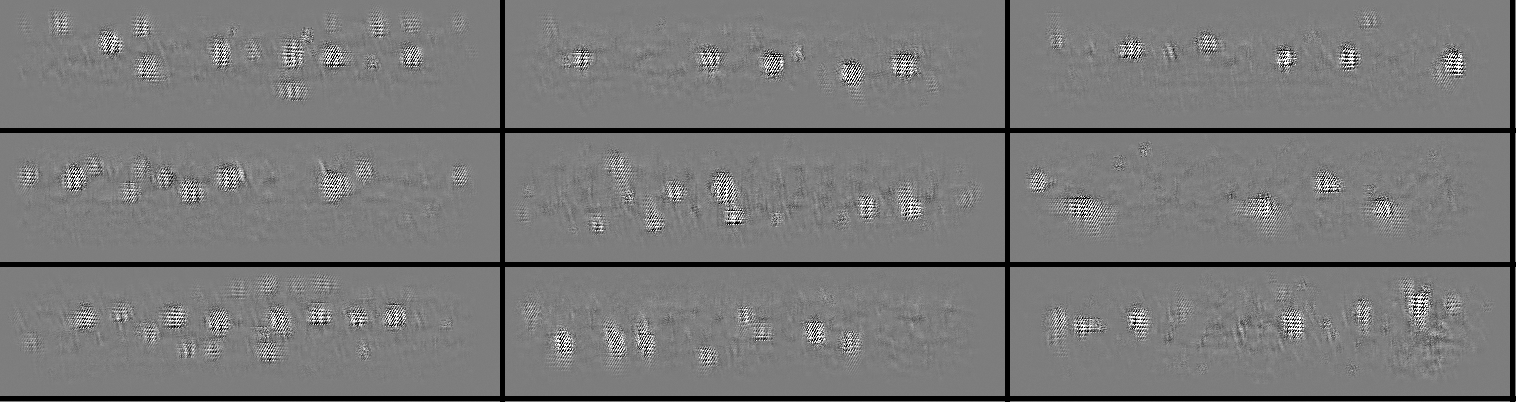
\includegraphics[width=\textwidth, keepaspectratio]{img/conv_filter.png}
    	\caption{Visualization of nine filters in the final convolutional layer. Note the ripple-like patterns responsible for detecting different frequency spans in the input audio.}
    	\label{fig:conv_filter}
	\end{figure}
%
To obtain these filters, we performed backpropagation from the output of each filter back to the input image. This yielded the gradients in the filter output with respect to the input image pixels. We used these to perform gradient ascent, searching for the image pixels that maximize the output of the filter, by following the method proposed by Chollet~\cite{chol16}.

Visualizations for the lower-level convolutional layers result in images of very simple geometric shapes like lines and circles, which matched our expectations. With increasing network depth, each convolutional layer's features combined and evolved into more complex shapes resembling our input domain. In Figure~\ref{fig:conv_filter}, we identify the familiar ripple-like patterns that represent frequency activations over time. This proves that the network learned these structures, as we hypothesized earlier. We can also identify that some filters specialize in high frequencies, whereas others focus on lower ones. Furthermore, it can be observed that the filters only react to a short and specific span of time within the spectrogram, all of which are less than one second long.

\subsubsection{Discussion}
\label{sec:comparison}
In this thesis, we introduced and compared different CNN and CRNN architectures for language identification and proved that these models can be used to solve our research task with a satisfying quality. Our evaluation confirms that audio tasks can be solved within the image domain using spectrogram image representations. As hypothesized, we were able to prove that our system learned the audio and frequency structures of these spectrogram images. We showed that these results are valid regardless of the input audio source and across various languages. Further, we demonstrated that the learned intermediate language representations were, indeed, universal and not language-specific and could easily be applied to other languages as well.

Our approach of combining convolutional neural networks with bidirectional long short-term memory cells showed a consistent improvement over baseline CNNs. In general, we were able boost accuracy significantly. Furthermore, we established that an Inception-v3-like CRNN outperformed all other approaches, both in terms of accuracy (\num{0.96}) as well as noise robustness.

We presented several augmented datasets to evaluate both robustness to noise and background music. We were content to note that the noise resistance of the Inception-v3 CRNN reached acceptable levels without us having to modify or restructure our algorithm. This reaffirms our belief in deep learning techniques as a viable tool for audio tasks.

Our CRNN approach interpreted every vector entry along the $x$ axis as a separate time step for the recurrent layer. Hence, all gathered results are representative of only ten-second snippets of the original audio files. We believe that we could increase the prediction performance in a production-ready system by issueing a majority vote across multiple segments of a longer audio file.
